\section{Ausgangslage}
\label{sec:Ausgangslage}

\begin{wrapfigure}{l}{0.55\textwidth}
  \begin{center}
    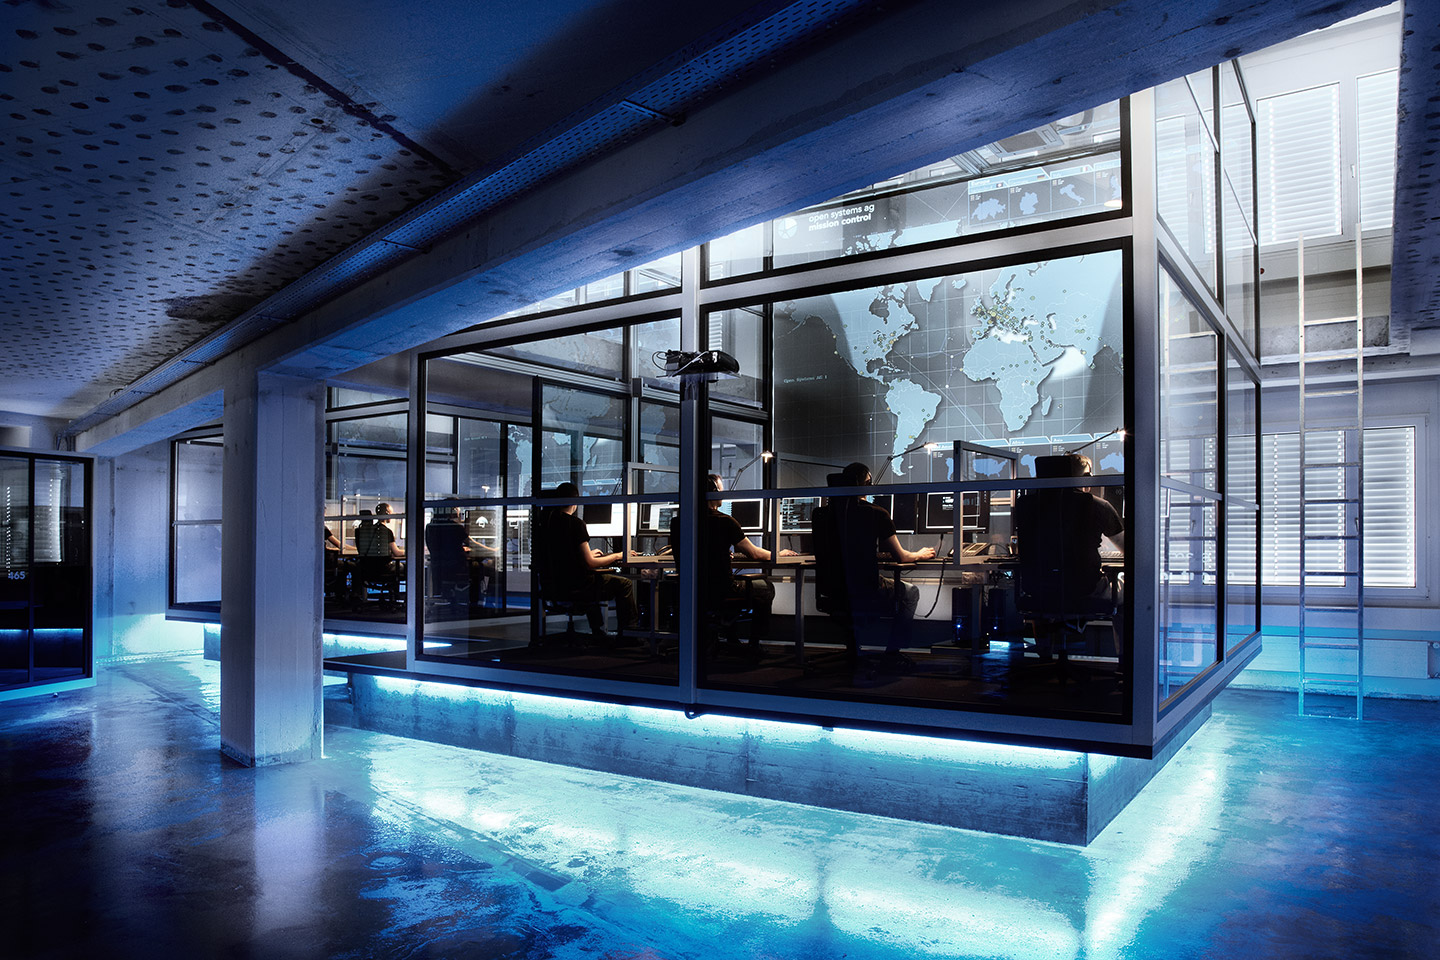
\includegraphics[clip,scale=0.15]{mainpart/anforderungen/img/gallery_mc_01}
    \caption{Mission Control Center}
  \end{center}
\end{wrapfigure}


Die Firma \osag{} betreibt ein weltweites Netz von \ac{IPsec} \ac{VPN} Verbindungen. Die Kunden der \osag{} kommen unter anderem aus den Branchen: Finanzen, Versicherungen, Regierung, NGO und Detail Handel. Daher ist es für die \osag{} sehr wichtig, dass die Verbindungen konstant überwacht werden. Zu diesem Zweck betreibt die \osag{} auch zwei Mission Control Center\footnotemark[1] mit den Standorten Zürich und Sydney. So ist ein \enquote{Follow-the-Sun} 24/7 Betrieb möglich.

\footnotetext[1]{Bild: \url{http://open.ch}}

Die Aufgabe dieser Mission Control Center ist es die \ac{VPN}-Verbindungen konstant zu überwachen und auftretende Probleme zu beheben. Anders als bei Firmen mit typischem First-, Second- und Third-Level Support sind die Mission Control Center stets von Ingenieuren besetzt, die auch schwierige Issues in kürzester Zeit lösen können. Für vermehrt vorkommende Probleme wird dort auch gleich eine automatisierten Lösung erstellt, sodass sie beim erneuten Auftreten nicht durch einen Menschen bearbeitet werden müssen.

Im Sinne dieser Automatisierungsbestrebung soll mit dieser Arbeit auch das Detektieren von Paket-Verlusten und die Bestimmung der \ac{MTU} gelöst werden.
Das manuelle Überprüfen von Paket-Verlusten und Bestimmen von Fragmentierungsproblemen nimmt viel Zeit in Anspruch. Es soll nun eine Applikation programmiert werden, womit sich diese Arbeit automatisieren lässt, sodass mit weniger Aufwand eine bessere Verbindungsqualität gewährleistet werden kann.


\subsection{Produktfunktion}
Es soll eine Applikation (\tool{}) entwickelt werden die das Erkennen und Diagnostizieren von Problemen bei \ac{IPsec} \ac{VPN}-Verbindungen vereinfacht.Dabei soll das Tool die Möglichkeit bieten passiv Paket-Verluste zu erkennen, sowie aktiv die \ac{MTU} zu bestimmen. Die Applikation wird als konstant laufender Service konzipiert und bietet daher keine grafische Oberfläche, sondern nur ein Commandline-Interface. Für die Kommunikation mit den Benutzern sollen Log-Einträge verwendet werden.

\subsection{Benutzercharakteristik}
Die Benutzer der Applikation sind Netzwerkadministratoren \& Informatik-Ingenieure die \ac{IPsec} \ac{VPN} Tunnels betreiben. Ein grosses Mass an technischem Verständnis und Erfahrung im Zusammenhang mit \ac{IPsec} und \ac{VPN}-Verbindungen kann deshalb vorausgesetzt werden. Sie haben ausgeprägte Kenntnisse in der Bedienung von Linux und Commandline-Applikationen.

\subsection{Abhängigkeiten}
Das Tool wird als eigenständige Applikation entwickelt und kann zur Fehlerdiagnose bei beliebigen \ac{IPsec} Tunnels eingesetzt werden. Es gibt keine enge Bindung zu externen Applikationen oder zur Infrastruktur der \osag{}.